\documentclass[conference]{IEEEtran}

\usepackage{verbatim}
\usepackage{framed}
\usepackage{flushend}
\usepackage{multirow}
\usepackage{graphicx}
\usepackage{rotating}

\newcommand{\codeinline}[1]{{\fontsize{8}{0}\selectfont\texttt{#1}}}
\newcommand{\codeintable}[1]{{\fontsize{6.215}{7.458}\selectfont\texttt{#1}}}
\newcommand{\codefile}[1]{
  \begin{framed}
  \fontsize{5.65}{6.78}\selectfont
  \verbatiminput{#1}
  \end{framed}
}

\begin{document}

\title{CSE6339 -- The Big Assignment\vspace{-14pt}}
\author{Yasser Gonzalez-Fernandez -- ygf@yorku.ca, ygonzalezfernandez@gmail.com\vspace{4pt} \\ March, 2014}

\maketitle


\begin{abstract}
Solutions to the second assignment of the course CSE6339 3.0 Introduction to Computational Linguistics. 
Instructor: Prof. Nick Cercone, Department of Electrical Engineering \& Computer Science, York University, Canada.
\end{abstract}


\section{Introduction}

The motivation for the assignment is illustrated in the following statement.
``If enough monkeys were allowed to pound away at typewriters for enough time, all the great works of literature would result''~\cite{Bennett1976}.
The typist monkeys in question represent a device 
-- in the assignment, a computer program -- 
capable of generating a random sequence of characters.

Computer simulation programs of different complexity are used, ranging from zero-order monkeys 
-- that generate all characters independently and with the same probability -- 
to programs using statistics of order greater than zero computed from writing samples.
The output of the programs is compared to the content of the literary work they are trying to reproduce in order to evaluate their performance.
The statistics computed from the writing samples are also used to perform author attribution and genre classification tasks.

The remainder of the report is organized as follows.
Firstly, Section~\ref{sec:documentation} describes the implementation of the programs created for the assignment.
Then, Section~\ref{sec:solutions} continues with the actual solutions to the nine problems.
Lastly, Section~\ref{sec:conclusions} summarizes the results and provides some concluding remarks.


\section{Program Documentation\label{sec:documentation}}

A collection of Python scripts were developed for the solution of the problems in the assignment.
Each individual script uses a group of common functionalities implemented in a main module called \codeinline{monkeys.py}.
In the code, external dependencies were kept at minimum by relying only on the Python Standard Library.
The rest of this section describes the most important data structures and algorithms used in \codeinline{monkeys.py}.
The complete source code of the module is included in an appendix at the end of the report.

\subsection{Preprocessing}

The distinction between upper and lower case characters is ignored in the assignment.
A total number of 40~different characters is considered: 
26~alphabetic characters folded to lower case (\codeinline{a}, \codeinline{b}, \codeinline{c}, \ldots, \codeinline{z}), 
13~punctuation marks (space, \codeinline{,}, \codeinline{.}, \codeinline{;}, \codeinline{:}, \codeinline{?}, \codeinline{!}, \codeinline{(}, \codeinline{)}, \codeinline{-}, \codeinline{'}, \codeinline{"}, \codeinline{@}),
and any digit (\codeinline{0}--\codeinline{9}) is counted as~\codeinline{\#}.
The \codeinline{map\_input\_char} function maps any input character in a writing sample to the characters considered in the assignment.
A character that do not appear among the 40~characters is mapped to~\codeinline{@} (in addition to~\codeinline{@} itself).

Additionally, an integer between 0 and 39 is assigned to each one of the 40~characters following the ASCII order
-- i.e. space~gets~0, \codeinline{!}~gets~1, \codeinline{"}~gets~2, \ldots, and \codeinline{z}~gets~39.
The functions \codeinline{char2index} and \codeinline{index2char} return the index corresponding to a given character and vice versa.
These indexes identify the entries of the frequency tables presented next in this section.

\subsection{N-Gram Frequency Tables}

Solving the problems in the assignment requires counting the occurences of all the character \mbox{\mbox{$n$-gram}s} appearing in a writing sample.
This section discusses how this information can be represented and the different operations that are needed.

\vspace{0.5em}
\subsubsection{Representation}

The most important data structure in the assignment is the \mbox{$n$-gram} frequency table, hereafter denoted by~$T$.
This table contains the frequency counts of every combination of $n$~characters over the alphabet of $m=40$ possible characters.
A particular entry $T_{c_1,\ldots,c_n}$ in the table can be identified by the indexes $c_1,\ldots,c_n \in [0,m-1]$ of the \mbox{$n$-gram} characters.
Also, if we follow the analogy of monkeys at typewriters, the entries $T_{c_1,\ldots,c_{n-1},k}, k=0,\ldots,m-1$ determine the layout of the typewriter corresponding to the \mbox{$n$-gram} prefix $c_1,\ldots,c_{n-1}$.

A table~$T$ is represented as a Python nested list with $n$~levels and $m$~entries per level.
This data structure is equivalent to a multidimensional $n \times m$ array, since Python lists are implemented as arrays of pointers in CPython.
This array-based representation guarantees O(1) read/write access to any particular entry in the table.
Based on this structure, the function \codeinline{compute\_freq\_tab} builds a frequency table of the specified order from a writing sample given as a collection of plain-text files.

One drawback of the array-based representation is that the table may contain many zero entries corresponding to \mbox{\mbox{$n$-gram}s} that never appeared on the writing sample.
A more memory-efficient implementation could have been based on a hash table (i.e. a Python dictionary) that stores only the \mbox{\mbox{$n$-gram}s} with nonzero frequencies.
Nevertheless, since only a maximum of third-order \mbox{\mbox{$n$-gram}s} are considered in the assignment, the more explicit array-based representation was preferred.
The more compact representation is however used to save the frequency tables to files on disk.
The function \codeinline{write\_freq\_tab} saves a mapping of the \mbox{$n$-gram} with nonzero frequencies as a JSON dictionary.
Consequently, the function \codeinline{read\_freq\_tab} reads a frequency table from a file in JSON format.


\vspace{0.5em}
\subsubsection{Most Probable Path}

Problem~1f (see Section~\ref{sec:problem1f}) requires using the procedure to compute the most probable path in a second-order frequency table described in the handout~\cite{Bennett1976}.
The function \codeinline{most\_probable\_freq\_tab\_path} implements a straightforward generalization of this algorithm for \mbox{\mbox{$n$-gram}s} with $n\geq2$.
Given an $n$-th order frequency table and a prefix of $n-1$~characters, the path is built incrementally by adding the character that completes the \mbox{$n$-gram} with the highest frequency at the end of the path.
The algorithm stops when all characters are already included in the path or an \mbox{$n$-gram} prefix with zero occurrences is found.

\vspace{0.5em}
\subsubsection{Reducing the Resolution}

For the solution of Problem~1d (see Section~\ref{sec:problem1d}), it is necessary a method to change the resolution of the frequency tables.
The function \codeinline{reduce\_freq\_tab\_resolution} achieves this purpose by reducing the number of keys on the typewriters.
If $F>0$ is the maximum frequency count in a table~$T$ of order~$n$, the entries of the reduced frequency table $T'$ are obtained as follows,

$$T'_{c_1,\ldots,c_n} = \left\lfloor\frac{T_{c_1,\ldots,c_n}}{\alpha F}\right\rfloor,$$

\noindent where $c_1,\ldots,c_n$ identify an entry in the table and $\alpha \in (0,1]$ is the reduction rate 
-- i.e. all entries are normalized by a fraction of the maximum frequency.
This method tries to preserve the relative proportions between frequencies that remain greater than zero after the transformation.


\vspace{0.5em}
\subsubsection{Simulation}

The function \codeinline{simulate\_freq\_tab} samples a number of characters following the distribution encoded in the frequency table.
If the argument corresponding to the frequency table is \codeinline{None}, the (zero-order) straightforward monkey problem is simulated.
For a frequency table of order~$n$, the first~$n-1$ characters are always sampled uniformly.
Also, a character is sampled uniformly if all the entries in the frequency table for the current \mbox{$n$-gram} prefix have zero frequencies in order to always satisfy the required number of characters.
The resulting string of characters is written to a plain-text output file.

The auxiliary function \codeinline{\_freq\_tab\_sample} is called from \codeinline{simulate\_freq\_tab} and it is responsible for sampling a single character given an \mbox{$n$-gram} prefix of $n-1$ characters.
The code in \codeinline{\_freq\_tab\_sample} first computes the list of cumulative frequencies for the entries corresponding to the \mbox{$n$-gram} prefix.
Then, an integer between zero and the cumulative sum of frequencies is sampled and its position in the cumulative list of frequencies determines the character to be returned.
Since the position of the can be determined in O($\log m$) using a bisection algorithm, the running-time for sampling a single character is O($m$) 
-- i.e. it is dominated by the computation of the cumulative frequencies.


\subsection{Evaluating the Output}

Some of the problems in the assignment require comparing the performance of different simulation programs.
Since the purpose is to reproduce a given literary work, the content of a file generated by \codeinline{simulate\_freq\_tab} is compared to the text of the book to be reproduced.
This comparison is performed in terms an evaluation measure calculated by the \codeinline{relative\_word\_yield} function.
The relative world yield is defined as the number correct words in the simulated file divided by the total number of words in the simulated file
-- a word is considered correct if it appears in the book to be reproduced.
In order to get a reasonable estimation of the performance measure, the simulated files contain ten times the number of characters in the book to be reproduced.

\subsection{Writing Sample Profiles}

The solutions to Problems 1g, 1h, and 1i use a technique called Common N-Gram (CNG) profiles~\cite{Keselj2003} to discover similarities between authors, and to perform author attribution and genre classification.
The function \codeinline{cng\_profile} builds a CNG profile of the specified length $L$ from a given frequency table.
A Python dictionary is used to represent the profile, as a mapping of the $L$ most-frequent \mbox{\mbox{$n$-gram}s} to their normalized frequencies.
Also, the function \codeinline{cng\_dissimilarity} computes a positive dissimilarity measure between two profiles.
The function returns zero for texts with identical $L$ most-frequent \mbox{\mbox{$n$-gram}s}.
For more information about the CNG profiles, please refer to the citation above.


\section{Solutions\label{sec:solutions}}

% (a) Readable listing of program, Programming style
% (b) Some sample outputs illustrating testing techniques
% (c) How to use program/system plus sample session


\subsection{Problem 1a}
\label{sec:problem1}

\begin{quote}
``Simulate the straightforward monkey problem. Let the program run long enough to 
give a meaningful estimate of the yield of words. The result will provide a 
useful comparison with later forms of the problem.''
\end{quote}

...the first book of each author listed in Table~\ref{tab:data} (books numbered~1, 
3, 4, 5, 6, 10, 11, 12, 14, 15, 19, 22, 23, 25, and 27)

\codefile{problem1a.py}

\begin{table}
\caption{Relative word yield of the straightforward monkey problem.\label{tab:problem1a}}
\vspace{-10pt}
\begin{center}
\begin{tabular}{cccc}
\hline
Book No. & Avg. Rate & Book No. & Avg. Rate \\
\hline
1  & 14.97\% & 14 & 7.88\% \\
3  & 26.55\% & 15 & 31.49\% \\
4  & 19.51\% & 19 & 34.18\% \\
5  & 31.02\% & 22 & 26.17\% \\
6  & 26.28\% & 23 & 14.91\% \\
10 & 25.13\% & 25 & 11.87\% \\
11 & 18.81\% & 27 & 13.91\% \\
12 & 17.71\% & & \\
\hline
\end{tabular}
\end{center}
\end{table}


\subsection{Problem 1b}
\label{sec:problem1b}

\begin{quote}
``Use the data in Table~\ref{tab:hamlet} to simulate the first-order monkey problem. 
Again let the program run long enough to give a meaningful estimate of the yield 
of words to permit comparison with other results on relative word yield. Try running
this simulation program against other corpora.''
\end{quote}

\begin{table}
\caption{\hspace{2em}Character Distribution from Act III of Hamlet. \newline
Note: 35,224 characters, a small corpus.\label{tab:hamlet}}
\vspace{-10pt}
\begin{center}
\begin{tabular}{crcrcr}
\hline
Char. & Freq. & Char. & Freq. & Char. & Freq. \\
\hline
space & 6,934  & r     & 1,593  & p     & 433   \\
e     & 3,277  & l     & 1,238  & b     & 410   \\
o     & 2,578  & d     & 1,099  & v     & 309   \\
t     & 2,557  & u     & 1,014  & k     & 255   \\
a     & 2,043  & m     & 889   & '     & 203   \\
s     & 1,856  & y     & 783   & j     & 34    \\
h     & 1,773  & f     & 629   & q     & 27    \\
n     & 1,741  & c     & 584   & x     & 21    \\
i     & 1,736  & g     & 478   & z     & 14    \\
\hline
\end{tabular}
\end{center}
\end{table}

\codefile{problem1b.py}

\begin{table}
\caption{Relative word yield of the first-order monkey problem \newline
with the character frequencies in Table~\ref{tab:hamlet}.\label{tab:problem1b}}
\vspace{-10pt}
\begin{center}
\begin{tabular}{cccc}
\hline
Book No. & Avg. Rate & Book No. & Avg. Rate \\
\hline
1  & 15.01\% & 14 & 7.89\% \\
3  & 22.35\% & 15 & 23.46\% \\
4  & 15.31\% & 19 & 24.94\% \\
5  & 23.50\% & 22 & 19.50\% \\
6  & 21.01\% & 23 & 14.68\% \\
10 & 21.89\% & 25 & 12.37\% \\
11 & 18.67\% & 27 & 17.40\% \\
12 & 15.51\% & & \\
\hline
\end{tabular}
\end{center}
\end{table}


\subsection{Problem 1c}
\label{sec:problem1c}

\begin{quote}
``Use the data supplied, data listed in Table~\ref{tab:data}, to simulate the 
second-order and third-order Bronte monkey problem. Again let the program run 
long enough to give a meaningful estimate of the yield of words to permit 
comparison with other results on relative word yield. Try running this 
simulation program against other authors listed.''
\end{quote}

\begin{table}
\caption{Data made available for the assignment.\label{tab:data}}
\vspace{-18pt}
\begin{center}
\begin{tabular}{r@{\hspace{1.1em}}l@{\hspace{1.1em}}l@{\hspace{0.75em}}r}
\hline
No. & Author & Title & Chars. \\
\hline
1  & C. Dickens & A Christmas Carol & 168,925 \\
2  & C. Dickens & A Tale of Two Cities & 773,928 \\
3  & E. Bronte & Wuthering Heights & 662,869 \\
4  & A. Bronte & Agnes Grey & 384,300 \\
5  & C. Bronte & Jane Eyre & 1,051,336 \\
6  & E. R. Burroughs & Tarzan of the Apes & 492,783 \\
7  & E. R. Burroughs & Warlord of Mars & 319,854 \\
8  & E. R. Burroughs & The People that Time Forgot & 212,736 \\
9  & E. R. Burroughs & The Land that Time Forgot & 205,762 \\
10 & H. R. Haggard & King Solomon's Mines & 454,437 \\
11 & J. Cleland & Fanny Hill & 474,725 \\
12 & L. Carroll & Alice's Adventures in Wonderland & 148,580 \\
13 & L. Carroll & Through the Looking Glass & 167,015 \\
14 & W. Irving & Legend of Sleepy Hollow & 69,164 \\
15 & Sir A. C. Doyle & The Adventures of Sherlock Holmes & 575,574 \\
16 & Sir A. C. Doyle & The Lost World & 432,766 \\
17 & Sir A. C. Doyle & The Hound of the Baskervilles & 327,348 \\
18 & Sir A. C. Doyle & Tales of Terror and Mystery & 421,264 \\
19 & M. Twain & Adventures of Huckleberry Finn & 578,345 \\
20 & M. Twain & The Adventures of Tom Sawyer & 397,076 \\
21 & M. Twain & A Connecticut Yankee in & 657,430 \\
   &          & King Arthur's Court & \\
22 & N. Machiavelli & The Prince & 286,854 \\
23 & H. G. Wells & War of the Worlds & 346,458 \\
24 & H. G. Wells & The Time Machine & 182,881 \\
25 & F. Kafka & Metamorphosis & 122,139 \\
26 & F. Kafka & The Trial & 462,372 \\
27 & R. Kipling & The Jungle Book & 279,771 \\
\hline
\end{tabular}
\end{center}
\end{table}

...the books written by the Bronte sisters in Table~\ref{tab:data}
(books numbered 3, 4, and 5).

\codefile{problem1c.py}

\begin{table}
\caption{Relative word yield of the second-order (2nd) and 
third-order (3rd) Bronte monkey problem.\label{tab:problem1c}}
\vspace{-10pt}
\begin{center}

\begin{tabular}{cccccr}
\hline 
\multirow{2}{*}{Book No.} & \multicolumn{2}{c}{Avg. Rate} & \multirow{2}{*}{Book No.} & \multicolumn{2}{c}{Avg. Rate} \\
\cline{2-3} \cline{5-6} 
 & 2nd & 3rd &  & 2nd & 3rd\hspace{0.75em} \\
\hline
1  & 24.78\% & 40.03\% & 14 & 18.57\% & 37.56\% \\
3  & 32.43\% & 44.57\% & 15 & 30.65\% & 41.72\% \\
4  & 27.70\% & 41.87\% & 19 & 35.89\% & 45.42\% \\
5  & 35.38\% & 45.97\% & 22 & 28.89\% & 40.63\% \\
6  & 29.42\% & 41.20\% & 23 & 26.02\% & 40.65\% \\
10 & 30.33\% & 42.09\% & 25 & 23.02\% & 38.12\% \\
11 & 26.16\% & 41.41\% & 27 & 26.94\% & 41.13\% \\
12 & 24.93\% & 38.88\% &    &    & \\
\hline
\end{tabular}
\end{center}
\end{table}


\subsection{Problem 1d}
\label{sec:problem1d}

\begin{quote}
``Investigate the effects of resolution on monkey literacy in the simulation. 
For example round off the matrix elements to the smallest number of places --
or use an equivalent means to reduce the number of keys on the typewriters.''
\end{quote}

...a book of medium size was selected among the books listed in Table~\ref{tab:data} 
(book number 4).

\codefile{problem1d.py}

Fig.~\ref{fig:problem1d} shows the results of the study.

\begin{figure}[!t]
\centering
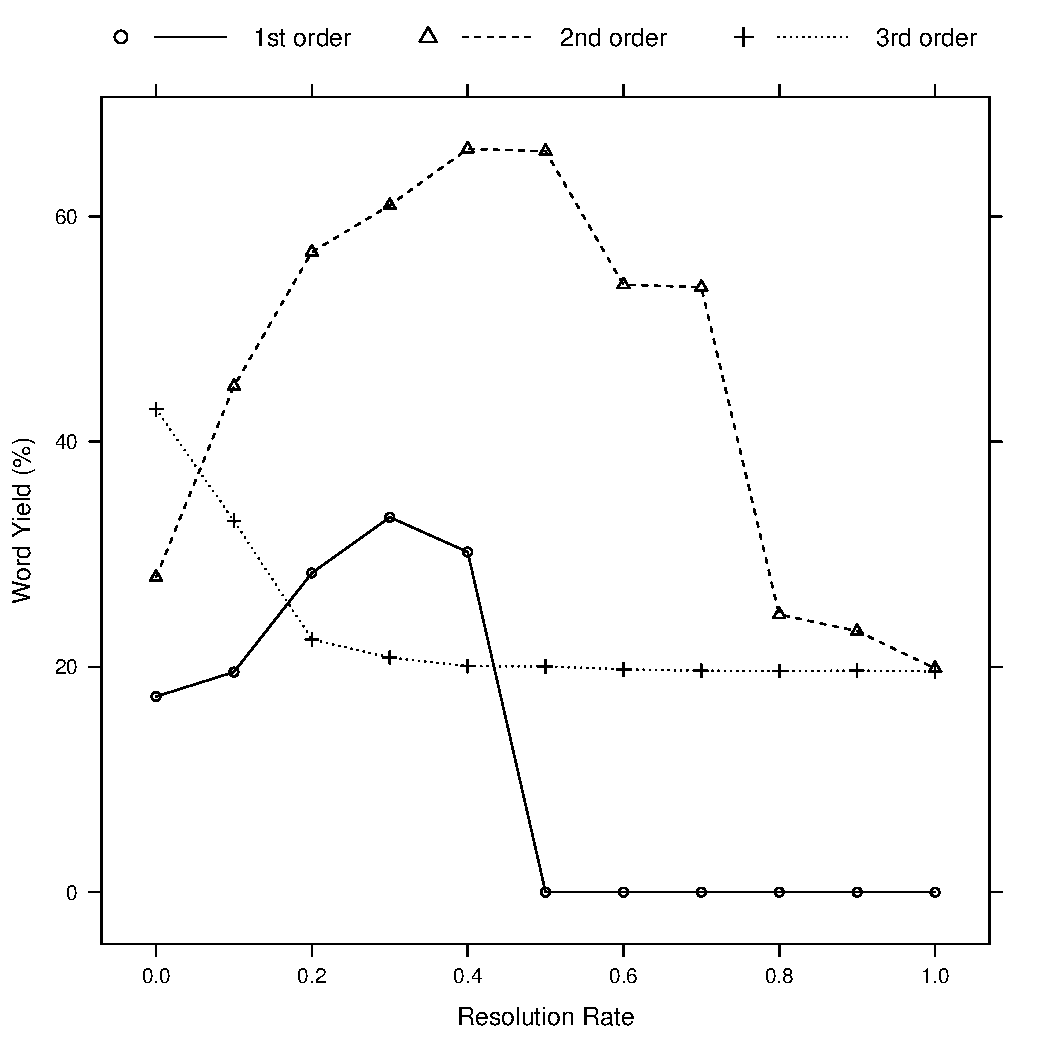
\includegraphics[width=3.4in]{problem1d}
\caption{Effect of resolution on monkey literacy.}
\label{fig:problem1d}
\end{figure}


\subsection{Problem 1e}
\label{sec:problem1e}

\begin{quote}
``Write a routine to compute correlation matrices of the type shown in the 
handout~\cite{Bennett1976} from data supplied (the books shown in Table~\ref{tab:data}).''
\end{quote}

\codefile{problem1e.py}

Figs.~\ref{fig:agnes_grey_2nd_order} and~\ref{fig:agnes_grey_3rd_order} show the results.

\begin{figure}[!t]
\centering
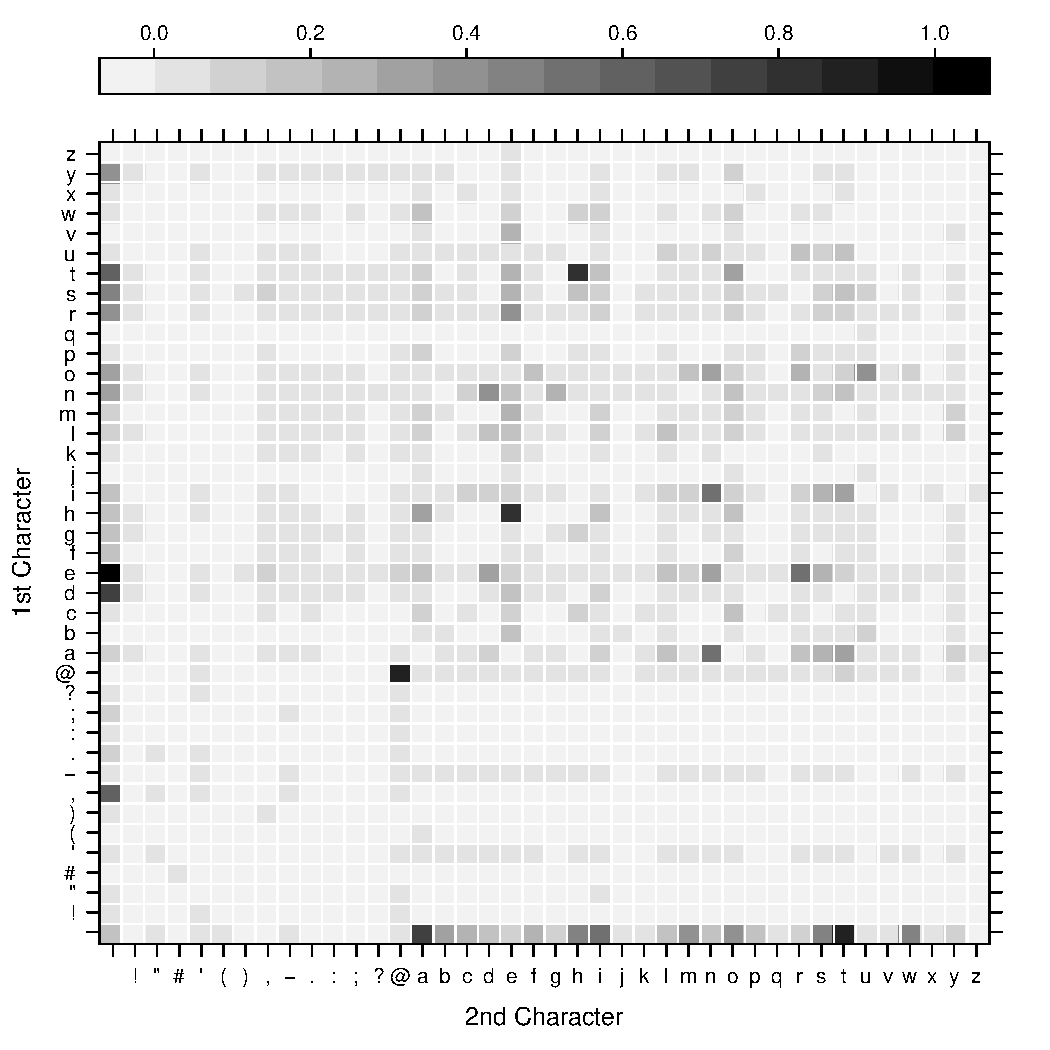
\includegraphics[width=3.4in]{agnes_grey_2nd_order}
\caption{Second-order correlation matrix built from A.~Bronte's ``Agnes Grey''.}
\label{fig:agnes_grey_2nd_order}
\end{figure}

\begin{figure*}[!t]
\centering
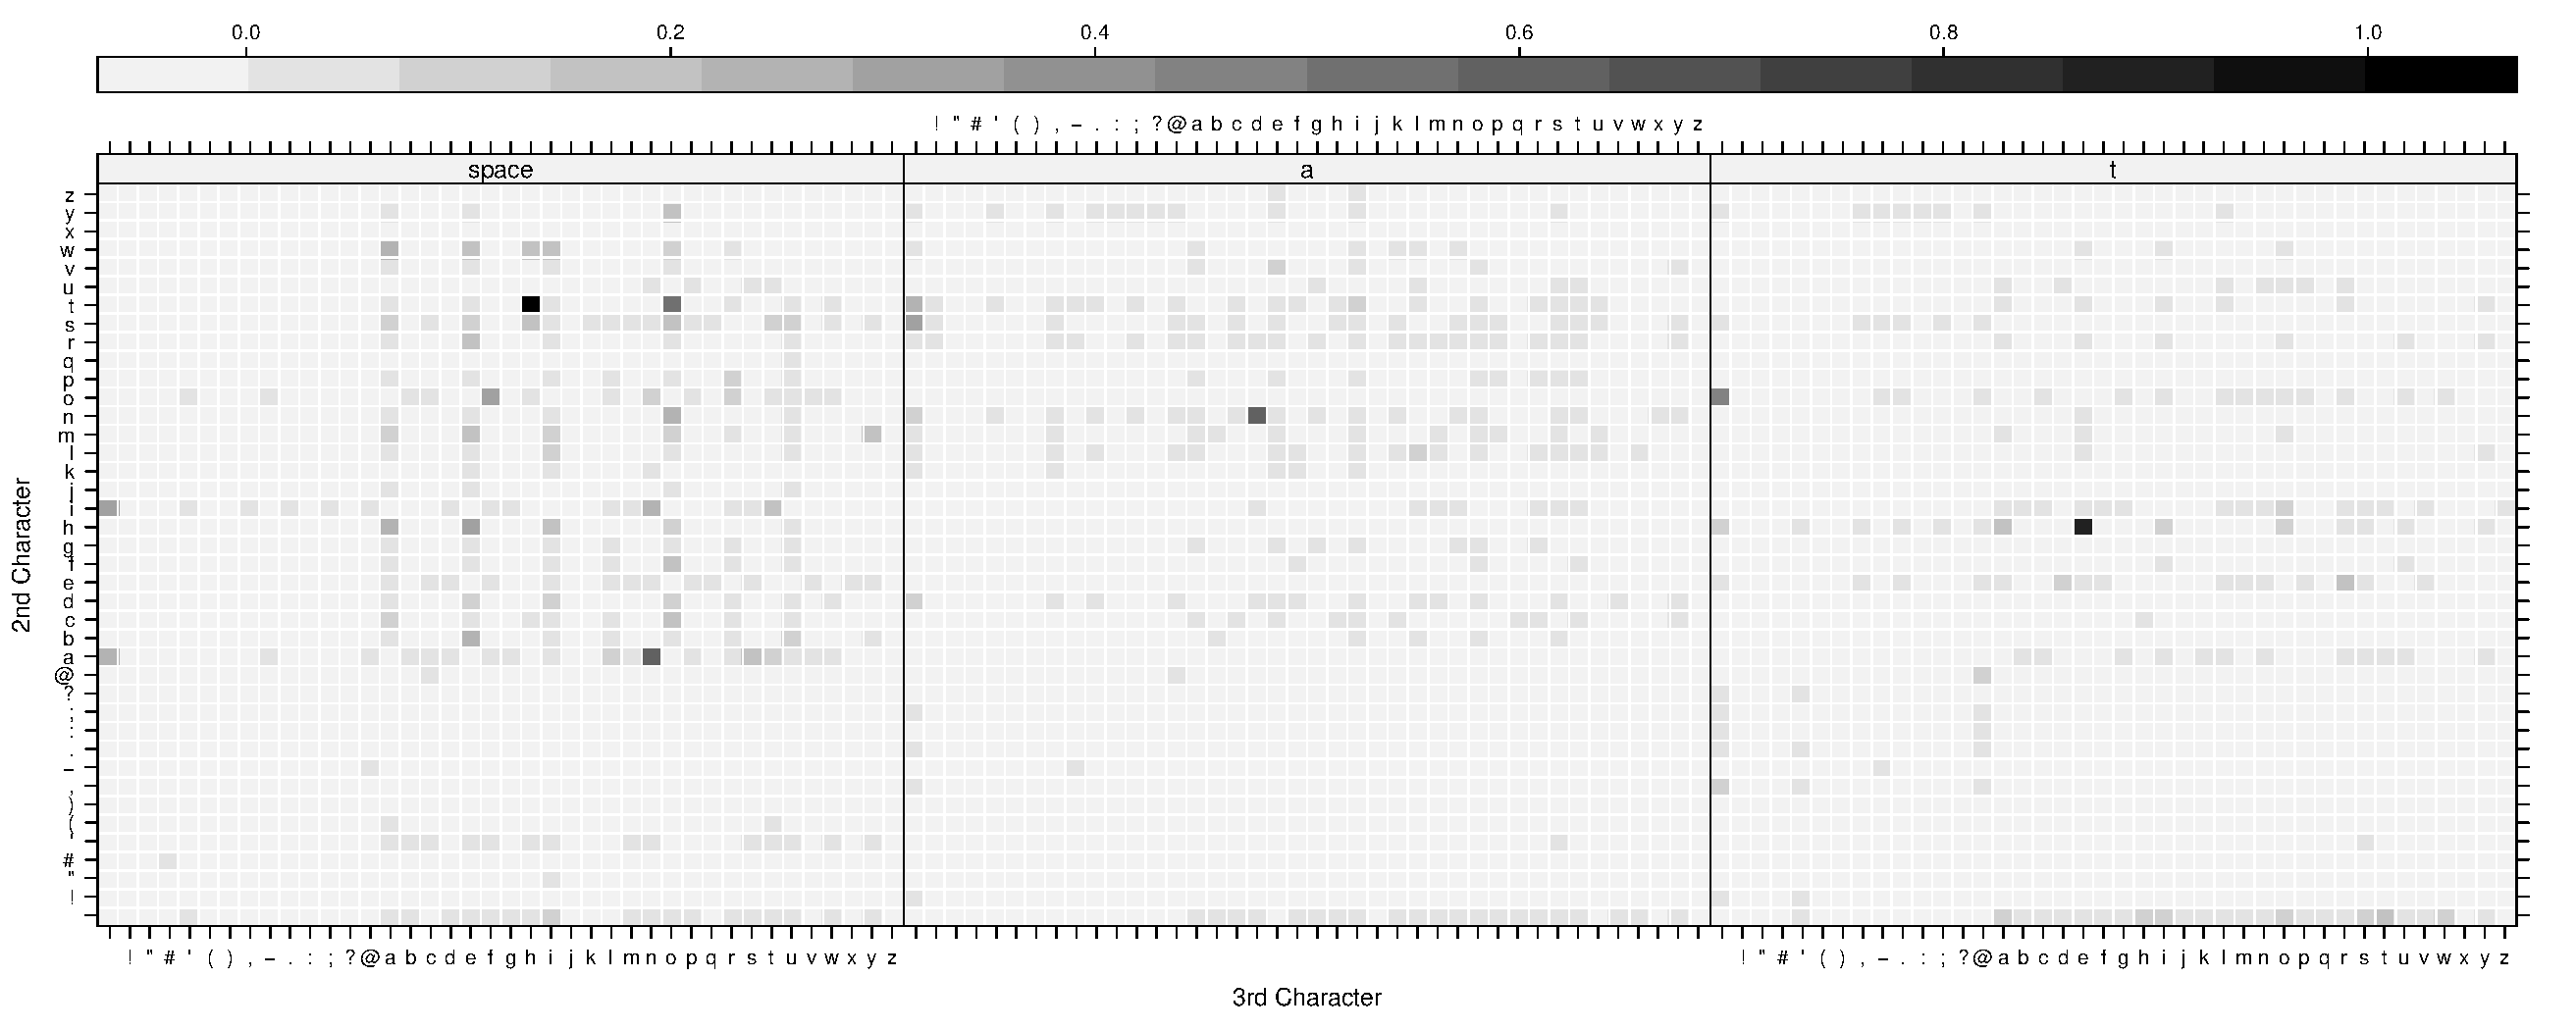
\includegraphics[width=\textwidth]{agnes_grey_3rd_order}
\caption{Selected entries of the third-order correlation matrix built from 
A.~Bronte's ``Agnes Grey''.}
\label{fig:agnes_grey_3rd_order}
\end{figure*}


\subsection{Problem 1f}
\label{sec:problem1f}

\begin{quote}
``Using the algorithm in the handout~\cite{Bennett1976} with the pair-correlation matrix 
generated from Irving (book shown in Table~\ref{tab:data}), compute the most 
probable digraph path, which starts with the letter `t'. Compare the result with 
that given in the handout for Poe's `The Gold Bug'''.
\end{quote}

\codefile{problem1f.py}

The book ``Legend of Sleepy Hollow'' by W. Irving (book number 14 in Table~\ref{tab:data}).
The most probable digraph is \codeinline{the andis,@wofry."bulmpk!-cq} and the 
trigraph \codeinline{the somplack,@}.

The most probable digraph path in Poe's ``The Gold Bug'' is: \codeinline{the andisouryplf'bj}.

\begin{table}
\caption{\hspace{2em}Most probable digraph (beginning with `t') and \newline 
trigraph (beginning with `th') paths.\label{tab:problem1f}}
\vspace{-10pt}
\begin{center}
\begin{tabular}{cll}
\hline 
\multirow{2}{*}{Book No.} & \multicolumn{2}{c}{Most Probable}  \\
\cline{2-3}
 & Digraph Path & Trigraph Path \\
\hline
1  & \codeintable{the andouscrimy,"@w.'lf-bj} & \codeintable{the said,"@} \\
3  & \codeintable{the andisour,'@cly."w-bj} & \codeintable{the and@,} \\
4  & \codeintable{the andisoury,@'w."blf-ck;} & \codeintable{the and@} \\
5  & \codeintable{the andisoury,@"w.'lf-bjp;} & \codeintable{the and@."-somplik} \\
6  & \codeintable{the andisorzly,"@w.'mpug-f?)} & \codeintable{the saingly,@} \\
10 & \codeintable{the and,"@siloury.'ck-bj} & \codeintable{the sompard,@\#} \\
11 & \codeintable{the andis,@wofry."bluck;} & \codeintable{the of@} \\
12 & \codeintable{the andoury,'@sicklf.)-bj} & \codeintable{the wasking,'@} \\
14 & \codeintable{the andis,@wofry."bulmpk!-cq} & \codeintable{the somplack,@} \\
15 & \codeintable{the andouris,"@w.'ckly-bj} & \codeintable{the and@} \\
19 & \codeintable{the andoulis,@"w.'mybrkf-g;} & \codeintable{the was@} \\
22 & \codeintable{the andis,@wory."culf-\#;(?)} & \codeintable{the and@} \\
23 & \codeintable{the andisofry,@wlup."g-mbj} & \codeintable{the somplack,@} \\
25 & \codeintable{the andouly,@simpr'v} & \codeintable{the was@} \\
27 & \codeintable{the andoulis,"@bry.)-ck!'mp?} & \codeintable{the was@,} \\
\hline
\end{tabular}
\end{center}
\end{table}


\subsection{Problem 1g}
\label{sec:problem1g}

\begin{quote}
``Design and implement an experiment using data from the books shown in Table~\ref{tab:data}
that might be used to perform author attribution. Discuss your solution and provide reasons 
why it is likely or not likely to solve the problem definitively.''
\end{quote}

The authors with more than one book listed in Table~\ref{tab:data} 
-- i.e. C. Dickens, E. R. Burroughs, L. Carroll, Sir A. C. Doyle, M. Twain, 
H. G. Wells, and F. Kafka -- were selected for the experiment and divided 
into two training/testing groups. A CNG profile was built for each author using 
all the books except the first one -- e.g. M. Twain's profile was built using 
`The Adventures of Tom Sawyer' and ``A Connecticut Yankee in King Arthur's Court''. 
Then, the first book by each author -- e.g. M. Twain's ``Adventures of Huckleberry Finn'' 
-- was considered for author prediction. The following Python code implements 
this experimental procedure:

\codefile{problem1g.py}

The results are shown in Table~\ref{tab:problem1g}.


\begin{table}
\caption{\hspace{1.4em}Results of the author attribution experiment using \newline
values of the GNG profile length $L\in\{10,100,500\}$.\label{tab:problem1g}}
\vspace{-10pt}
\begin{center}
\begin{tabular}{lr@{\hspace{1em}}r@{\hspace{1em}}r}
\hline 
\multirow{2}{*}{Correct Author} & \multicolumn{3}{c}{Predicted Author}\tabularnewline
\cline{2-4} 
 & $L=10$ & $L=100$ & $L=500$\tabularnewline
\hline
C. Dickens & C. Dickens & C. Dickens & C. Dickens \\
E. R. Burroughs & E. R. Burroughs & E. R. Burroughs & E. R. Burroughs \\
L. Carroll & M. Twain & L. Carroll & L. Carroll \\
Sir A. C. Doyle & M. Twain & Sir A. C. Doyle & Sir A. C. Doyle \\
M. Twain & M. Twain & M. Twain & M. Twain \\
H. G. Wells & C. Dickens & E. R. Burroughs & H. G. Wells \\
F. Kafka & F. Kafka & F. Kafka & F. Kafka \\
\hline
Prediction Rate & 57.14\% & 85.71\% & 100.00\%\\
\hline
\end{tabular}
\end{center}
\end{table} 
    

\subsection{Problem 1h}
\label{sec:problem1h}

\begin{quote}
``Can you develop a metric based on what you have done so far to classify the stories, e.g., 
as mystery, romance, action/adventure, etc.? Implement your techniques to demonstrate 
classification. Can the classification scheme you designed help with author attribution? 
Can you say something about correlations among books written by the same author? 
Is there any relationship to the styles of the three Bronte sisters' works?''
\end{quote}

\codefile{problem1h.py}

A dendrogram of the results is presented in Fig.~\ref{fig:problem1h}.

\begin{figure*}[!t]
\centering
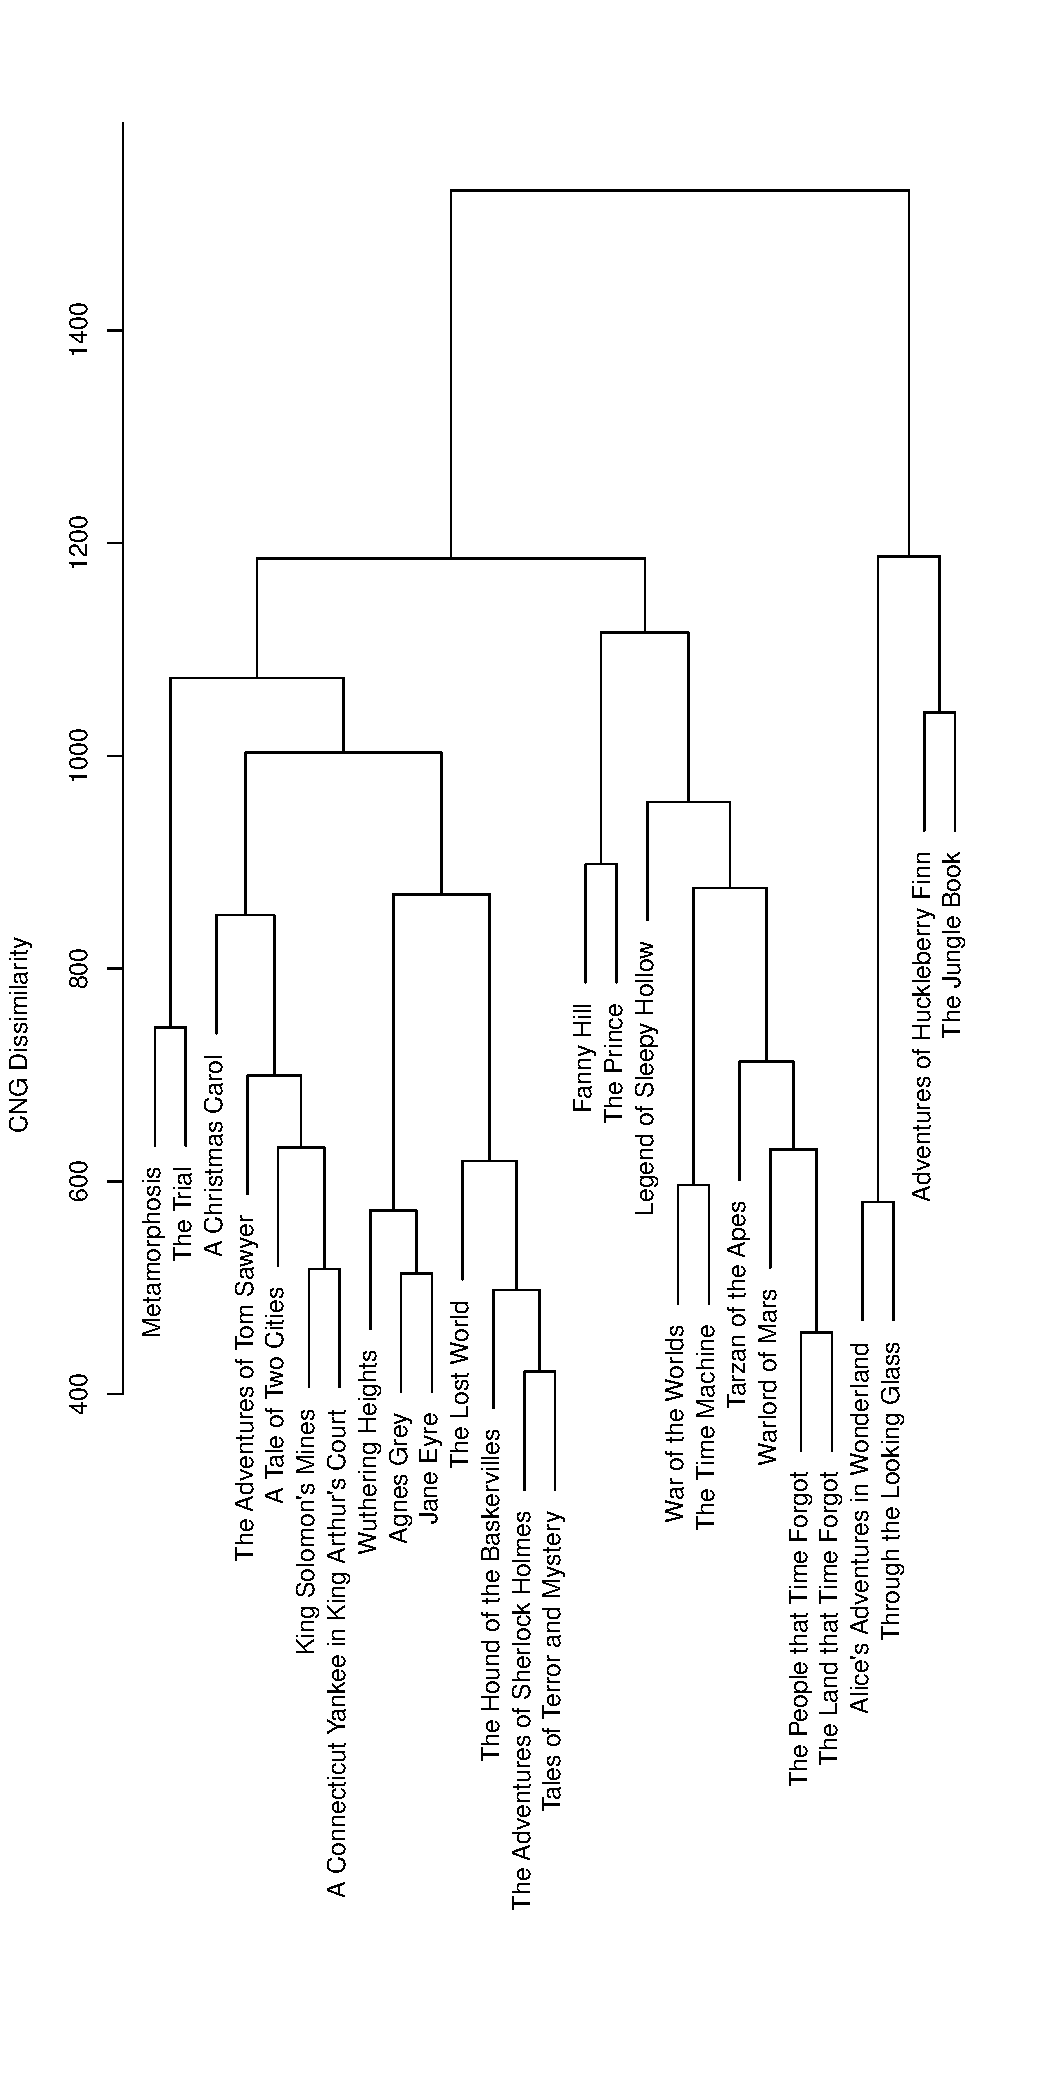
\includegraphics[height=\textwidth,angle=270]{problem1h}
\caption{Hierarchical cluster analysis of the data made available for the assignment
according to the CNG dissimilarity.}
\label{fig:problem1h}
\end{figure*}

\subsection{Problem 1i}
\label{sec:problem1i}

\begin{quote}
``Develop a profile for each of the different authors in Table~\ref{tab:data} and provide 
a metric and argument that compares and contrasts authors in order to speculate which 
two authors are the most `similar' in style.''
\end{quote}

\codefile{problem1i.py}

The CNG normalized dissimilarity matrix is presented in Table~\ref{tab:problem1i}.

\begin{table*}

\caption{\hspace{6em}Normalized CNG dissimilarity scores for every pair of authors. For each author, \newline
the score corresponding to its most similar counterpart is highlighted bold.\label{tab:problem1i}}
\vspace{-10pt}
\renewcommand{\arraystretch}{1.5}
\begin{center}
\begin{tabular}{r|ccccccccccccccc}
 & \begin{sideways}
C. Dickens
\end{sideways} & \begin{sideways}
E. Bronte
\end{sideways} & \begin{sideways}
A. Bronte
\end{sideways} & \begin{sideways}
C. Bronte
\end{sideways} & \begin{sideways}
E. R. Burroughs~
\end{sideways} & \begin{sideways}
H. R. Haggard
\end{sideways} & \begin{sideways}
J. Cleland
\end{sideways} & \begin{sideways}
L. Carroll
\end{sideways} & \begin{sideways}
W. Irving
\end{sideways} & \begin{sideways}
Sir A. C. Doyle
\end{sideways} & \begin{sideways}
M. Twain
\end{sideways} & \begin{sideways}
N. Machiavelli
\end{sideways} & \begin{sideways}
H. G. Wells
\end{sideways} & \begin{sideways}
F. Kafka
\end{sideways} & \begin{sideways}
R. Kipling
\end{sideways}\tabularnewline
\hline 
C. Dickens & $-$ & 0.52 & 0.48 & 0.41 & 0.46 & 0.47 & 0.60 & 0.79 & 0.60 & \textbf{0.34} & 0.49 & 0.67 & 0.55 & 0.56 & 0.64 \\
E. Bronte & 0.52 & $-$ & 0.41 & \textbf{0.37} & 0.56 & 0.63 & 0.62 & 0.75 & 0.73 & 0.52 & 0.60 & 0.76 & 0.64 & 0.63 & 0.79 \\
A. Bronte & 0.48 & 0.41 & $-$ & \textbf{0.37} & 0.56 & 0.54 & 0.51 & 0.72 & 0.70 & 0.49 & 0.53 & 0.66 & 0.60 & 0.53 & 0.77 \\
C. Bronte & 0.41 & \textbf{0.37} & \textbf{0.37} & $-$ & 0.48 & 0.49 & 0.53 & 0.81 & 0.67 & \textbf{0.37} & 0.51 & 0.70 & 0.54 & 0.60 & 0.73 \\
E. R. Burroughs & 0.46 & 0.56 & 0.56 & 0.48 & $-$ & 0.43 & 0.59 & 0.85 & 0.58 & \textbf{0.35} & 0.54 & 0.69 & 0.44 & 0.65 & 0.67 \\
H. R. Haggard & 0.47 & 0.63 & 0.54 & 0.49 & 0.43 & $-$ & 0.65 & 0.78 & 0.59 & \textbf{0.39} & 0.42 & 0.70 & 0.47 & 0.66 & 0.60 \\
J. Cleland & 0.60 & 0.62 & \textbf{0.51} & 0.53 & 0.59 & 0.65 & $-$ & 0.96 & 0.65 & 0.58 & 0.73 & 0.64 & 0.64 & 0.74 & 0.87 \\
L. Carroll & 0.79 & 0.75 & 0.72 & 0.81 & 0.85 & 0.78 & 0.96 & $-$ & 1.00 & 0.81 & \textbf{0.66} & 1.00 & 0.87 & 0.73 & 0.83 \\
W. Irving & 0.60 & 0.73 & 0.70 & 0.67 & \textbf{0.58} & 0.59 & 0.65 & 1.00 & $-$ & 0.60 & 0.73 & 0.72 & \textbf{0.58} & 0.79 & 0.84 \\
Sir A. C. Doyle & \textbf{0.34} & 0.52 & 0.49 & 0.37 & 0.35 & 0.39 & 0.58 & 0.81 & 0.60 & $-$ & 0.48 & 0.67 & 0.46 & 0.53 & 0.65 \\
M. Twain & 0.49 & 0.60 & 0.53 & 0.51 & 0.54 & \textbf{0.42} & 0.73 & 0.66 & 0.73 & 0.48 & $-$ & 0.81 & 0.57 & 0.56 & 0.56 \\
N. Machiavelli & 0.67 & 0.76 & 0.66 & 0.70 & 0.69 & 0.70 & \textbf{0.64} & 1.00 & 0.72 & 0.67 & 0.81 & $-$ & 0.76 & 0.78 & 0.93 \\
H. G. Wells & 0.55 & 0.64 & 0.60 & 0.54 & \textbf{0.44} & 0.47 & 0.64 & 0.87 & 0.58 & 0.46 & 0.57 & 0.76 & $-$ & 0.71 & 0.70 \\
F. Kafka & 0.56 & 0.63 & \textbf{0.53} & 0.60 & 0.65 & 0.66 & 0.74 & 0.73 & 0.79 & \textbf{0.53} & 0.56 & 0.78 & 0.71 & $-$ & 0.75 \\
R. Kipling & 0.64 & 0.79 & 0.77 & 0.73 & 0.67 & 0.60 & 0.87 & 0.83 & 0.84 & 0.65 & \textbf{0.56} & 0.93 & 0.70 & 0.75 & $-$ \\
\end{tabular}
\end{center}
\end{table*} 


\section{Conclusions\label{sec:conclusions}}

% The Python source code of the programs implemented for the assignment is available at the git repository \codeinline{https://github.com/ygf/monkeys-typing}.
% The repository also contains the \LaTeX~code for this document, and the R~scripts and data files to produce the accompanying figures.


\bibliographystyle{IEEEtran}
\bibliography{references,IEEEabrv}

\appendix[Source Code of the `monkeys.py' Module]

\codefile{monkeys.py}

\end{document}
